\documentclass[10pt]{article}

%\usepackage{hyperref}
\usepackage{alltt}
\usepackage{natbib}
\usepackage{graphicx}
\usepackage{url}
\usepackage{fancyhdr}
\usepackage{trust}
\pagestyle{fancy}

\lhead{}
\rhead{}
\lfoot{\copyright The University of Kansas, 2012}
\cfoot{\thepage}


\newtheorem{conjecture}{Conjecture}
\newtheorem{obligation}{Obligation}
\newtheorem{definition}{Definition}


\usepackage{ifthen}
\newboolean{submission}  %%set to true for the submission version
\setboolean{submission}{false}
%\setboolean{submission}{true}
\ifthenelse
{\boolean{submission}}
{ \newcommand{\todo}[1]{ } } % hide todo
{ \newcommand{\todo}[1]{ % show todo
   \marginpar{\raggedright\footnotesize{#1}}
               }}

\parskip=\medskipamount
\parindent=0pt

\bibliographystyle{abbrvnat}

\title{Attestation Protocols: A Tutortial Introduction}
\author{Perry Alexander \and Brigid Halling}

\begin{document}

\maketitle
\tableofcontents
\listoffigures
\listoftables

\begin{abstract}
  This document is intended to provide a tutorial overview of the
  basic attestation protocols used by a TPM.
\end{abstract}

\section{Introduction}

\section{Certificate Authority Based Attestation}

\begin{enumerate}
  \parskip=0pt\itemsep=0pt
\item An appraiser sends an attestation request indicating what PCRs
  are needed along with a nonce.

\item The user software receives the request and requests a fresh AIK
  key pair from the TPM using the \verb+TPM_MakeIdentity+ command.
  Parameters to the \verb+TPM_MakeIdentity+ command describe
  properties of the desired AIK pair.

\item The TPM responds to the \verb+TPM_MakeIdentity+ command by
  generating a new AIK wrapped key pair and returning the public key,
  \public{AIK} signed by the TPM using \private{AIK}.  The new AIK is
  installed in the TPM prior to signing it's public part.

\item The user software sends the certified public EK and the signed
  public \public{AIK} to the Privacy CA.  The public AIK is signed by
  the TPM using \private{AIK}.

\item The Privacy CA checks the certificate on EK and determines if it
  has been revoked.  It then uses \public{AIK} to check the signature
  on itself.  Recall that only the TPM with AIK installed could
  generate that signature.  If signature check succeeds, the Privacy
  CA knows the key is from the right TPM.  If both checks are
  successful, the Privacy CA signs a certificate for the public AIK
  and encrypts the certificate with a fresh session key.  It they
  encrypts the session key and the public AIK with EK.

\item Both the encrypted certificate and the encrypted session key and
  AIK are receive by the user software.  The user software then uses
  the \verb+TPM_ActivateIdentity+ command to decyrpt the session key.
  Only the TPM associated with EK can decrypt the session key and will
  in turn decrypt the certificate.  Thus, any recipient of the
  certificate knows the AIK was generate by the right TPM.

\item The user software decrypts the AIK certificate with the session
  key that can only be obtained if it has access to the TPM associated
  with the public EK sent to the CA.

%% Quote needs to contain the nonce.

\item The user software requests a quote from the TPM using the
  \verb+TPM_Quote+ command.  The resulting quote is signed with the
  AIK.  The certified AIK public key is also signed with the AIK.  The
  user software sends the signed AIK certificate, signed quote, and
  stored measurement list back to the appraiser.

\item The appraiser analyzes the signed blobs received from the user
  software as follows: (i) the certified public AIK is used to check
  it's own signature; (ii) the certified public AIK is used to check
  the quote signature; (iii) the nonce is checked against the nonce
  sent with the request; and (iv) PCRs from the quote are compared
  with expected values.
\end{enumerate}

\begin{figure}
  \centering
  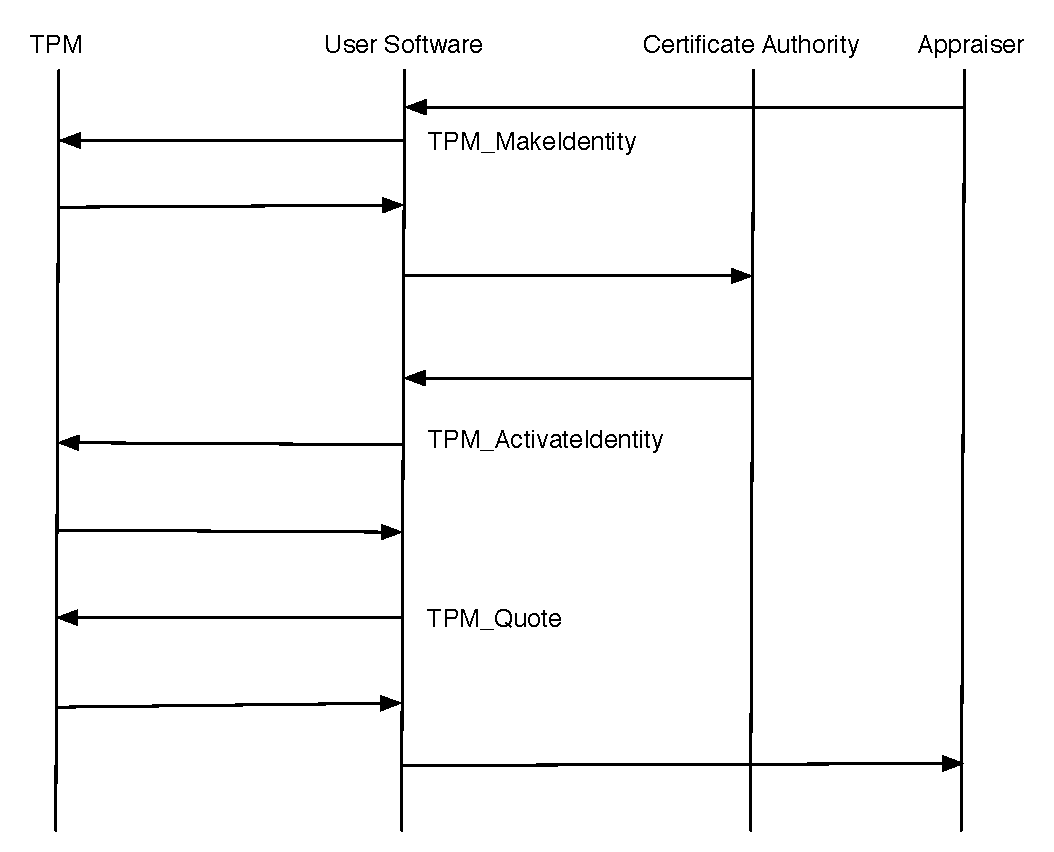
\includegraphics[width=0.75\textwidth]{figures/ca-attestation.pdf}
  \caption{Protocol for Privacy CA remote attestation.}
  \label{fig:ca-attestation}
\end{figure}


\section{Direct Anonymous Attestation}

\bibliography{attestation}

\end{document}
